\documentclass[12pt]{article}
\usepackage{ctex}
\usepackage[english]{babel}
\usepackage{blindtext}
\usepackage{nameref}
\usepackage{fancyhdr}
\usepackage{amsmath,amssymb,amsthm}
\usepackage{graphicx,float}
\usepackage{physics}
\usepackage{pgfplots}
\usepackage[a4paper, total={6in, 9in}]{geometry}

\graphicspath{{../image/}}

\pagestyle{fancy}
\fancyhf{}
\fancyhf[HL]{微分幾何1:向量與導數}
\fancyhf[CF]{\thepage}

\newcommand{\innerprod}[2]{\langle{#1},{#2}\rangle}
\newcommand{\id}{\mathtt{id}}

\newtheorem{definition}{定義}
\newtheorem*{theorem}{定理}
\newtheorem*{corollary}{衍理}
\newtheorem*{lemma}{引理}
\newtheorem*{proposition}{命題}
\newtheorem*{remark}{小記}
\newtheorem*{claim}{主張}
\newtheorem*{example}{示例}
\newtheorem*{axiom}{公設}
\renewenvironment*{proof}{\textit{證明.}}{\hfill$\qed$}

\newenvironment*{sol}{\par \textbf{解}.}{\hfill$\blacksquare$}

\begin{document}
    References: Introduction to Real Analysis (Bartle \& Sherbert), Thomas Calculus 12th Edition
    \section*{向量}

    向量屬於一種特殊的矩陣,通常用以表達\textbf{多維坐標}。

    \begin{definition}[向量]
        一個\textbf{$n$-維向量}包含$n$個元素,可視之爲\textbf{$n$-維空間}中的坐標,同時代表從原點指向該坐標的箭頭。
    \end{definition}
    
    爲方便描述,記$V_S$為帶有$S$域的元素的向量集合。

    \begin{definition}[向量加法]
        在向量集合$V_S$中,若$\vec{x}=(x_i)_i=(x_1,x_2,\dots),\vec{y}=(y_i)_i=(y_1,y_2,\dots)\in V_S$,則$$\vec{x}+\vec{y}:=(x_1+y_1,x_2+y_2,\dots)=(x_i+y_i)_i$$
    \end{definition}

    \begin{definition}[標量乘法]
        在向量集合$V_S$中,若$\vec{x}=(x_i)_i=(x_1,x_2,\dots)\in V_S$,$\alpha \in S$,則$$\alpha \vec{x}:=(\alpha x_1,\alpha x_2,\dots)=(\alpha x_i)_i$$
    \end{definition}
    \section*{向量空間}

    \begin{definition}[向量空間]
        設$V_S$為向量集合,且$\vec{x},\vec{y},\vec{z}\in V_S$, $\alpha, \beta \in S$。若$V_S$符合以下定理:\begin{itemize}
            \item 加法結合律:$(\vec{x}+\vec{y})+\vec{z}=\vec{x}+(\vec{y}+\vec{z})$。
            \item 加法交換律:$\vec{x}+\vec{y}=\vec{y}+\vec{z}$。
            \item 加法單位元:$\vec{0}\in V_S$使得$\vec{x}+\vec{0}=\vec{0}+\vec{x}=\vec{x}$。
            \item 加法逆:$\forall \vec{x}\in V_S$, 存在$\vec{y}\in V_S$使得$\vec{x}+\vec{y}=\vec{y}+\vec{x}=\vec{0}$。
            \item 標乘結合律:$\alpha(\beta \vec{x})=(\alpha\beta)\vec{x}$。
            \item 標乘單位元:$1\in S$使得$1\vec{x}=\vec{x}$。
            \item 分配律1:$\alpha(\vec{x}+\vec{y})=\alpha\vec{x}+\alpha\vec{y}$。
            \item 分配律2:$(\alpha+\beta)\vec{x}=\alpha\vec{x}+\beta\vec{x}$。
        \end{itemize}
    \end{definition}

    \begin{example}
        $\mathbb{R}$是一個向量空間。而且任何域也是一維向量空間。
    \end{example}

    \begin{example}
        在牛頓力學中討論力時,我們會以向量表示力的大小與方向。假設目前的討論僅限於平面(二維空間),並記施力點為原點$O$。
        \begin{figure}[H]
            \centering
            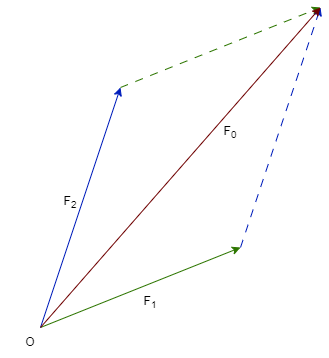
\includegraphics[scale=0.6]{Force.png}
        \end{figure}
        在上圖中可通過改變力量發生的先後次序來實現向量的平移,從而得出$$F_0=F_1+F_2$$的關係式。
    \end{example}

    \section*{向量函數}

    \section*{偏導數與全導數}

    \section*{方向導數}

    \section*{切面與法綫}

    \section*{二維極值與鞍點}
\end{document}